\begin{frame}
  \frametitle{Nuclear Security and Forensics}
  \begin{minipage}{0.6\textwidth}
    \begin{figure}
      \centering
      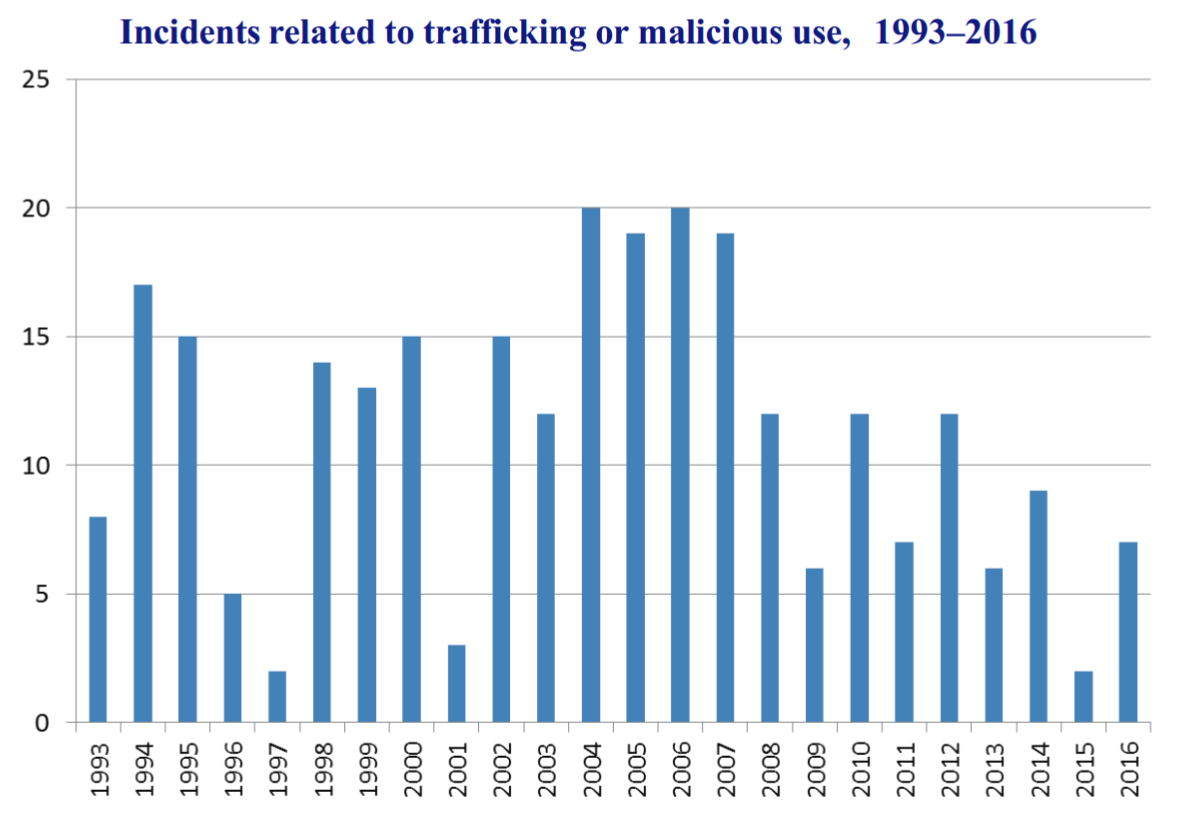
\includegraphics[width=\textwidth]{./figures/nucleartrafficking.png}
      \caption{24 years of incidents: HEU (12), Pu (2), Pu-Be neutron sources (4)
               \tiny [Obtained from:
               \url{https://www.iaea.org/sites/default/files/17/12/itdb-factsheet-2017.pdf}]}
    \end{figure}
  \end{minipage}%
  \begin{minipage}{0.4\textwidth}
    \begin{itemize}
      \item FY2016 DHS DNDO budget : 0.3 bill
      \item FY2016 DOE NNSA nonpro budget : 1.6 bill
    \end{itemize}
  \end{minipage}
\end{frame}

\begin{frame}
  \frametitle{Needs in Nuclear Forensics}
  \begin{figure}
    \centering
    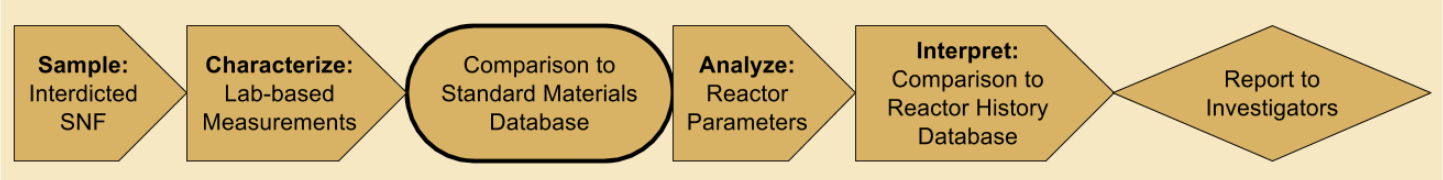
\includegraphics[width=\textwidth]{./figures/forensicsrealworld.png}
    \caption{Typical techincal nuclear forensics workflow}
  \end{figure}
  \begin{minipage}[t]{0.5\textwidth}
    Material-specific:
    \begin{itemize}
      \item Measurement needs
      \item Measurement techniques
      \item Forensic signatures
    \end{itemize}
  \end{minipage}%
  \begin{minipage}[t]{0.5\textwidth}
    Challenges:
    \begin{itemize}
      \item Rapid characterization
      \item Forensics databases
      \begin{itemize}
        \item Multidimensional
        \item Inconsistent uncertainties
        \item International cooperation
      \end{itemize}
    \end{itemize}
  \end{minipage}
\end{frame}

